% ZenGrowth field note — arXiv working paper v0.4.
% Adapted from the ZenInvest house template (docs/templates/zeninvest-arxiv/).
% Build: latexmk -pdf main.tex   (or pdflatex + bibtex + pdflatex x2)
% Style: self-contained single-column preprint layout (no external .sty).
%
% STATUS: v0.4 contains no first-hand measured figures. Each unmeasured
% claim maps to a procedure in docs/ACADEMIC-PUBLICATION-PLAN.md. Ground rule: never
% fabricate a statistic — "unmeasured" is written where data does not exist.
% Literature rechecked through 2026-08-26; product pages last verified 2026-07.
% Product pages document vendor claims, not independent outcome evidence.
\documentclass[11pt]{article}

\usepackage[utf8]{inputenc}
\usepackage[T1]{fontenc}
\usepackage{lmodern}
\usepackage{microtype}
\usepackage[margin=1.1in]{geometry}
\usepackage{booktabs}
\usepackage{tabularx}
\usepackage{float}
\usepackage{graphicx}
\usepackage{tikz}
\usetikzlibrary{arrows.meta,positioning,fit,calc}
\usepackage[numbers,sort&compress]{natbib}
\usepackage{xcolor}
\usepackage{url}
\usepackage[colorlinks=true,linkcolor=blue!60!black,citecolor=blue!60!black,urlcolor=blue!60!black]{hyperref}
\hypersetup{
  pdftitle={Grounded, Not Automated: A Verification-First LLM Career System},
  pdfauthor={Kayvan Nejabati Zenouz},
  pdfsubject={Working system, capability evidence, and prospective evaluation},
  pdfkeywords={LLM, career tools, human oversight, grounding, auditability}
}
\usepackage{titlesec}
\titleformat*{\section}{\large\bfseries}
\titleformat*{\subsection}{\normalsize\bfseries}

\newcommand{\gbp}{\pounds}
\definecolor{zgink}{RGB}{28,55,82}
\definecolor{zgfill}{RGB}{241,245,249}
\definecolor{zggate}{RGB}{90,40,40}
\definecolor{zgok}{RGB}{28,72,52}

\title{\textbf{Grounded, Not Automated: A Verification-First LLM Career System}}

\author{%
  Kayvan Nejabati Zenouz\\
  ZenGrowth (ZENOUZ.ai)\\
  \texttt{zenouz.ai@gmail.com}%
}

\date{August 2026\\[0.5em]\normalsize Working paper v0.4 --- working system and
prospective evaluation; comparative measurements pending}

\begin{document}
\maketitle

\begin{abstract}
AI career tools promise more interviews through resume optimization or
unattended application volume, usually without audited outcome denominators.
We present ZenGrowth, a working, audience-of-one, local-first system used in a
live senior AI/Data-Science search. One repository connects compliant role
discovery, inspectable scoring, evidence-grounded application materials,
interview preparation, offer evaluation, and lifecycle records. Its design
constrains generation to a reviewed evidence bank, rejects selected
unallowlisted numbers and named entities, records instrumented model calls,
and requires operator approval for every outbound artifact. The implementation
and regression tests establish capability-level evidence: these workflow and
control mechanisms exist and execute. They do not establish comparative speed,
sentence-level factual entailment, or improved callback rates. We therefore
separate demonstrated functionality from process and outcome claims, and
prospectively specify audits of grounding, score stability, review and elapsed
time, cost, and downstream outcomes. The current contribution is practical as
well as methodological: a coherent, operator-controlled application workflow,
a falsifiable evaluation protocol, and a claim-audit checklist. Our working
hypothesis is deliberately modest: supervised drafting can be useful when
errors remain reviewable, while autonomous submission moves model errors into
an irreversible, reputation-bearing action.
\end{abstract}

\section{Introduction}

Between 2023 and 2026 the AI job-search category split into two promises.
The first is \emph{optimization}: score your resume against a job
description and close the keyword gap (Jobscan's Match Rate, Teal's Match
Score)~\citep{jobscan2026, tealhq2026}. The second is \emph{automation}:
agents that discover postings and submit applications with minimal human
involvement, at volumes of hundreds per week~\citep{jobcopilot2026,
aihawk2026}. Both promises are typically supported by testimonials and
vendor-reported statistics rather than denominator-complete outcome audits.

ZenGrowth is a system built inside this category but against its grain. It
automates everything \emph{except} the send: discovery, explainable scoring,
evidence-grounded document generation, interview preparation, and offer
evaluation --- with a verification path that makes several high-risk forms of
fabrication mechanically detectable, and a human-approval boundary that makes
every outbound artifact the operator's deliberate act. It is also an
audience-of-one deployment: built by its operator for a live senior
AI/Data-Science search, with workflow events and instrumented model costs logged.

That combination --- category-typical capability, category-atypical
verification, and an inspectable audit trail --- is what makes an honest field
note possible. This paper asks three questions. (1)~What useful functionality
does the working repository already establish (\S\ref{sec:deployment})?
(2)~Which claims about smoothness, speed, correctness, and outcomes still need
measurement (\S\ref{sec:deployment})? (3)~Where do LLMs genuinely add value in
the job search, given the evidence behind category claims
(\S\ref{sec:claims}--\S\ref{sec:recommendations})?

\section{Relation to prior work}
\label{sec:priorwork}

Candidate-side LLM systems are no longer absent from the literature.
ResumeFlow generates job-specific resumes from a source resume and proposes
task-specific alignment and hallucination metrics~\citep{zinjad2024resumeflow}.
Resume Tailor is the closest \emph{longitudinal case study}: a career vault,
multi-source retrieval, provenance tracking, guardrails, and a conditional
review loop across nine job descriptions, with ATS-style fit-score
deltas~\citep{abhinav2026career}. Grounded Optimization is the closest
\emph{method} paper on rewrite defenses: a five-layer stack (temporal
validation, deterministic contamination detection, structural invariants,
prompt-level grounding, and an evaluator agent) with ablations on 25
synthetic resumes, reducing detected hallucinations from 2.48--5.36 per resume
in undefended baselines to 0.04--0.24~\citep{indukuri2026grounded}. These
results already occupy the ``add grounding gates'' slot. They do not audit a
live search, measure operator correction burden, or report
denominator-complete downstream outcomes.

Synapse takes the opposite design bet: evolutionary, LLM-guided resume
mutation to raise recommender and screening scores~\citep{erol2026synapse}.
That is a useful foil. ZenGrowth treats score-chasing as a failure mode
(\S\ref{sec:taxonomy}), not as an objective.

ConFit~v3 studies the adjacent matching problem with multi-pass LLM re-ranking,
listwise training, data cleaning, and distillation on real-world person--job
fit datasets~\citep{yu2026confit}. It strengthens benchmark evidence for
matching and ranking; it does not establish that an integrated candidate
workflow is faster, more accurate, or more effective.

Attune shows a newer human--AI direction for text-record scoring: users can
inspect and deterministically edit criteria and rules derived from pairwise
comparisons~\citep{chopra2026attune}. Its formative study ($n=12$), technical
evaluation, and domain-expert study ($n=8$) make rationale-bearing scoring
alone a weak novelty claim. ZenGrowth does not implement Attune's interactive
criteria steering; its narrower opportunity is to measure score stability,
operator disagreement, and correction burden in a live candidate workflow.

ZenGrowth's remaining proposed delta is therefore \emph{operational}: a live,
local-first deployment that connects reviewed evidence, deterministic
write-time risk gates, cost and latency telemetry, an application-level action
log, and a hard approval boundary between reversible assistance and
reputation-bearing send. Unlike an ATS-style fit score, its planned evaluation
treats unsupported or embellished claims after review as the primary failure
outcome, and reports operator time as part of the return rather than a free
safety layer. That delta is a hypothesis until the audits in
\S\ref{sec:deployment} are complete.

In the broader agent literature, ZenGrowth is not a new general-purpose agent
architecture or benchmark. AgencyBench evaluates long-horizon capability over
138 tasks and 32 real-world scenarios~\citep{li2026agencybench}. Auditable
Agents already formalizes action recoverability, lifecycle coverage, policy
checkability, responsibility attribution, and evidence integrity
\citep{nian2026auditable}. ZenGrowth should be read as a domain-specific
implementation and evaluation opportunity, not as the origin of agent
auditability. Interview research with 17 experienced developers identifies a
priori control, co-planning, real-time monitoring, and post hoc review as
distinct forms of oversight~\citep{dhanorkar2026oversight}. ZenGrowth currently
emphasizes a priori gates and post hoc operator review; it does not yet
evaluate the other forms or show that its review is sufficient.
Recent work on audit-budget allocation further shows why self-reported model
confidence is an unsafe basis for selective review when confidence is
miscalibrated or errors are correlated~\citep{zavattari2026auditbudget}.

Employer-side work provides important context but not evidence that
candidate-side tailoring improves outcomes. In two recruitment-platform field
experiments, shortlisted candidates assessed with AI interview information
passed a blind final human interview 17.5--20 percentage points more often than
candidates shortlisted from resumes alone; however, 75\% of invitees did not
complete the AI interview, shifting screening cost to applicants
\citep{aka2026bettertogether}. This is evidence for a different intervention,
not for resume rewriting or application agents. Classical correspondence
experiments manipulate perceived identity in otherwise similar
applications~\citep{bertrand2004emily}. More recent audits
find demographic sensitivity in embedding retrieval and GPT-based resume
assessment~\citep{wilson2024resume,armstrong2024silicon}; a 2026 audit across
newer models reports null or reversed gaps in several settings, showing that
direction and magnitude depend on model vintage and protocol~\citep{gao2026hire}.
Other 2026 counterfactual audits find disparities from subtle sociocultural
markers and gender effects in Japanese-format resumes, reinforcing that
anonymization, prompting, language, and task design materially affect an audit
result~\citep{tan2026smallchanges,hoffstedde2026japanese}.
Nor does a human-in-the-loop label guarantee correction: in a controlled
resume-screening experiment ($N=528$), participants followed simulated biased
AI recommendations up to 90\% of the time, including in some conditions where
they judged the recommendations low quality or unimportant
\citep{wilson2025nothoughts}.
The relevant conclusion is not that all screeners share one stable bias, but
that candidate materials enter a model-mediated environment whose behavior
requires versioned, task-specific auditing, and that human approval must itself
be evaluated rather than assumed sufficient.

\section{Capability evidence: the working ZenGrowth deployment}
\label{sec:deployment}

\subsection{The system under test}

ZenGrowth is a local-first FastAPI/React application with a SQLite store,
operated since early 2026 for a live senior AI/DS search. Its pipeline:
nightly compliant discovery over public ATS feeds (Greenhouse/Lever JSON;
no scraping of job boards) with a dead-man's-switch heartbeat; an LLM-free
relevance precheck; single-call strict-JSON scoring that records a
per-dimension rationale and a \emph{priority score} --- a weighted sum of
observable fit dimensions in which the model's uncalibrated
success-probability guess is demoted to a tie-breaking band and application
effort is a separate cost axis; and evidence-grounded generation of CVs,
cover letters, and application answers. Interview packs, transcript debriefs,
offer evaluation, and onboarding/departure planning use the same pattern:
research and drafting with provenance, never dispatched by the system.

The verification path is the load-bearing component (Figure~\ref{fig:architecture}).
Source documents are parsed into claims with provenance; claims auto-verify
only when the cited span exists in the source and high-risk tokens match that
span, while the rest queue for operator review. Generation receives only
verified claims. Write-time gates reject numbers and a conservative subset of
named entities found in neither the evidence bank nor the job context. These
allowlists catch important fabrication classes --- invented figures, uncited
employers --- but do not prove that every sentence is entailed by its cited
evidence; that stronger property is the subject of the planned claim-level
audit. Alias resolution merges entity surface variants. A deterministic,
zero-LLM-cost JD match report (term coverage, quantified-line count, clich\'e
detection) accompanies every material as a signal, not a target. Drafts carry
a never-sent banner until the operator acts.

Instrumented model paths record cost and latency; a configured daily spend
ceiling fails closed; and meaningful workflow transitions land in an
audit log streamed to the dashboard. The continuously integrated test suite
includes deterministic eval gates: hard-fact faithfulness, retrieval recall,
entity-resolution pairwise F1, claim-versus-span distortion checks, and a
scoring calibration suite (rewording stability bounds, hand-ranked
monotonicity, anchor drift alarms) --- all CI-enforced with zero LLM spend.

Scoring is \emph{model-aware}. Older Anthropic models may receive an explicit
\texttt{temperature=0} as a reproducibility request. Current production
defaults to Claude Sonnet~5, which rejects non-default sampling parameters;
the client omits temperature rather than send an invalid request. Neither
choice guarantees identical provider outputs. Repeated-score stability is
therefore a measured quantity, not an assumed property of the API. Sonnet~5's
new tokenizer also prevents direct reuse of earlier token and cost baselines;
model, tokenizer, pricing date, and token counts must be frozen together
\citep{anthropic2026sonnet5}.

\begin{figure}[t]
\centering
\resizebox{\linewidth}{!}{%
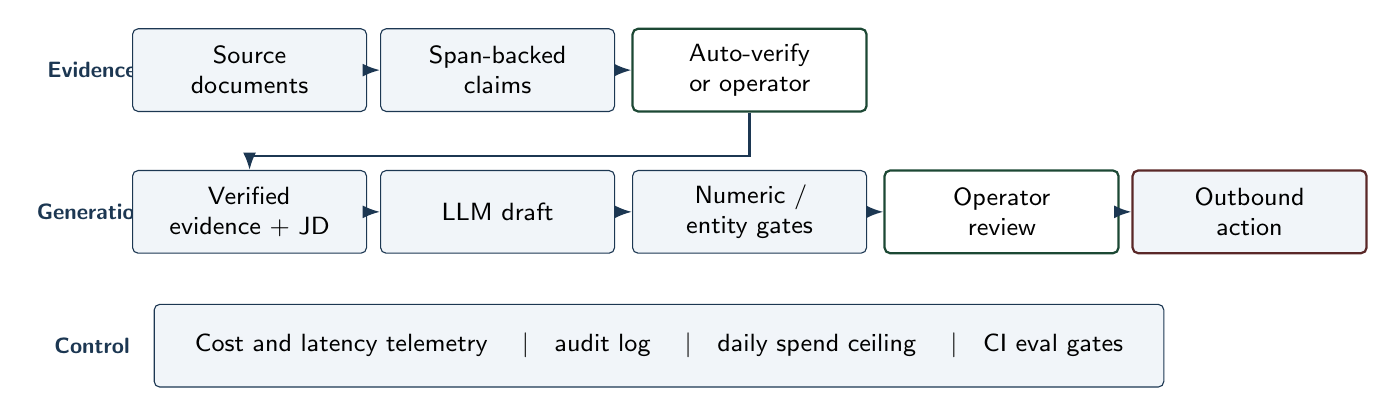
\begin{tikzpicture}[
  font=\small\sffamily,
  box/.style={draw=zgink, fill=zgfill, rounded corners=2pt, align=center,
    inner xsep=6pt, inner ysep=5pt, text width=2.55cm, minimum height=1.05cm},
  op/.style={box, fill=white, draw=zgok, thick},
  arr/.style={-{Latex[length=2.2mm]}, zgink, thick},
  lane/.style={font=\footnotesize\bfseries\sffamily, zgink}
]
\node[lane] (l1) at (0,2.35) {Evidence};
\node[box] (src) at (2.0,2.35) {Source\\documents};
\node[box] (clm) at (5.15,2.35) {Span-backed\\claims};
\node[op] (ver) at (8.35,2.35) {Auto-verify\\or operator};
\draw[arr] (src) -- (clm);
\draw[arr] (clm) -- (ver);

\node[lane] (l2) at (0,0.55) {Generation};
\node[box] (ctx) at (2.0,0.55) {Verified\\evidence + JD};
\node[box] (llm) at (5.15,0.55) {LLM draft};
\node[box] (gat) at (8.35,0.55) {Numeric /\\entity gates};
\node[op] (rev) at (11.55,0.55) {Operator\\review};
\node[box, draw=zggate, thick] (out) at (14.7,0.55) {Outbound\\action};
\draw[arr] (ctx) -- (llm);
\draw[arr] (llm) -- (gat);
\draw[arr] (gat) -- (rev);
\draw[arr] (rev) -- (out);
\draw[arr] (ver.south) -- ++(0,-0.55) -| (ctx.north);

\node[lane] (l3) at (0,-1.15) {Control};
\node[box, text width=12.4cm] (ctl) at (7.2,-1.15)
  {Cost and latency telemetry \quad$\vert$\quad audit log
   \quad$\vert$\quad daily spend ceiling \quad$\vert$\quad CI eval gates};
\end{tikzpicture}%
}
\caption{Verification-first pipeline. Evidence is verified before generation.
Deterministic gates catch selected token classes. Only the operator may
cross into an outbound action. The control plane records spend and workflow
transitions so later aggregates are diagnosable.}
\label{fig:architecture}
\end{figure}

\subsection{Capability evidence and the utility boundary}

The repository is more than an architectural proposal or a collection of
prompts: it runs an integrated workflow whose outputs remain inspectable by its
operator. Table~\ref{tab:capabilities} distinguishes that demonstrated
functionality from the comparative claims that begin with measurement.

\begin{table}[H]
\centering
\footnotesize
\begin{tabularx}{\linewidth}{>{\raggedright\arraybackslash}p{0.20\linewidth}>{\raggedright\arraybackslash}p{0.33\linewidth}>{\raggedright\arraybackslash}X}
\toprule
\textbf{Capability} & \textbf{Repository evidence} & \textbf{Defensible current claim} \\
\midrule
Find and prioritize & Feed adapters, deterministic precheck, rationale-bearing score & Working intake and prioritization; not proven relevance or ranking benefit \\
Prepare materials & Reviewed claim bank, provenance, numeric/entity gates & Reviewable, evidence-bounded drafting; not complete semantic correctness \\
Continue the process & Interview, offer, onboarding, and departure modules & One evidence trail across stages; not measured effort reduction \\
Control and diagnose & Never-send boundary, telemetry, spend ceiling, audit events & Operator-controlled and inspectable operation; not proof every error is caught \\
\bottomrule
\end{tabularx}
\caption{Capability evidence ladder. The working repository supports the
claims in the final column now; speed, smoothness, correctness rates, and
downstream outcomes require the prospective evaluation below.}
\label{tab:capabilities}
\end{table}

This is the paper's present utility claim: ZenGrowth supplies useful
functionality for organizing and executing a job-application workflow while
keeping external action under human control. Whether it makes that workflow
smoother or faster, how often its drafts remain correct after review, and
whether it improves application outcomes are separate empirical questions.

\subsection{Prospective evaluation and current status}

Table~\ref{tab:pending} is a claims scorecard, not a results table. The
repository establishes that the listed mechanisms exist and are tested; it
does not establish their field rates or downstream value. Measurements will
be frozen as dated aggregate artifacts using the public protocol
\citep{zengrowth2026protocol} before numerical claims enter the abstract.

\begin{table}[H]
\centering
\footnotesize
\begin{tabularx}{\linewidth}{p{0.08\linewidth}p{0.34\linewidth}X}
\toprule
\textbf{Claim} & \textbf{Current verdict} & \textbf{Required measurement} \\
\midrule
C3/C7 & \textbf{Partially verified}: gates exist; semantic fidelity unmeasured & Precision-targeted, stratified pilot of $\geq$75 claims; pre-/post-review grounded, unsupported, and embellished rates with exact intervals \\
C4 & \textbf{Unmeasured}: ``about two minutes'' withdrawn pending timing & All eligible runs in a frozen window (target $\geq20$); wall-clock split into wait, model, review, and correction \\
C5 & \textbf{Unmeasured}: per-call telemetry exists & Per-application cost distribution with operation inclusion rules and currency conversion date \\
C2/C8 & \textbf{Partially verified}: rationale exists; sampling is model-aware & $\geq10$ frozen postings with five repeats per model/version; score and rank variance \\
C1 & \textbf{Unmeasured}: discovery pipeline exists & Archive audit with relevance rubric, sample size, and relevant-role loss rate \\
C6 & \textbf{Partially verified}: local store and documented model egress & Enumerated egress audit: payload class, recipient, trigger, retention, and disclosure \\
C2b & \textbf{Unmeasured}: usefulness of rank unknown & Rank association with pre-specified pursue decisions; report $n$ and dependence limitations \\
--- & \textbf{Unmeasured}: callback/interview effect & Tracked campaign with complete application denominator and outcome follow-up \\
\bottomrule
\end{tabularx}
\caption{Claim status and prospective measurement plan for v1.}
\label{tab:pending}
\end{table}

\subsection{What the working repository already demonstrates}

Some findings do not wait for the quantitative pass because they are
architectural facts with test witnesses. The grounding gates fail generation
when a detectable, unallowlisted figure or entity appears, and the distortion
check demotes extracted claims whose numbers do not match their cited span.
Scoring records a rationale and applies sampling parameters only when the
named model accepts them. A configured daily ceiling blocks further model
calls once recorded spend reaches the cap. These are properties of the
implementation, not estimates of end-to-end factual accuracy, scoring
stability, or user value. The system is also \emph{diagnosable}: logged
workflow transitions and instrumented model costs make the planned aggregate
analyses possible. That auditability supported the diagnosis of
ranking-formula and lifecycle defects during development, while the
completeness of the log remains something to test rather than assume. The
evidence ladder is therefore explicit: working capability is established by
implementation and tests; process benefit is currently qualitative; effect
size, error rate, time saving, and downstream value remain unmeasured.

\subsection{Limitations of our evidence}
\label{sec:limitations}

A single operator, a single live search, one configuration lineage, no
control arm (no paired untailored applications), and small $n$ throughout;
the operator is also the system's author, so pursue-decisions are not
independent of the scoring being evaluated. Downstream outcomes confound
with market conditions, seniority, and field. The grounding audit samples
materials generated for real applications and therefore cannot be published
raw --- only aggregate, de-identified rates. Grounded Optimization already
reports rewrite-defense rates on synthetic resumes~\citep{indukuri2026grounded};
this paper cannot import those rates as field performance. These limitations
bound the claims: our data will support ``measured properties of one audited
deployment, with diagnosed mechanisms,'' not effect sizes for the category.

\section{The AI-career-tool claims landscape}
\label{sec:claims}

\emph{Qualitative synthesis from primary product pages accessed in 2026-07.
Product-defined match scores and vendor outcome claims are treated as marketing
evidence, not causal estimates. Academic neighbors were rechecked through
2026-08-26.}

\subsection{Optimization tools: scores without outcome audits}

Jobscan recommends a product-defined Match Rate of at least 75\%; Teal exposes
a 0--100\% resume-to-job score and emphasizes keyword and skill
alignment~\citep{jobscan2026,tealhq2026}. Both publish outcome-oriented claims,
but the reviewed pages do not disclose assignment mechanisms,
denominator-complete cohorts, attrition, or independent audits. Their scores
may be useful editing signals, but they are not calibrated callback
probabilities. Classical correspondence studies supply controlled callback
evidence for employer discrimination~\citep{bertrand2004emily}; they do not
identify the causal effect of commercial match-score optimization for the same
candidate. Systems that mutate a resume to raise a screener's score
\citep{erol2026synapse} inherit this conflation unless they also report
unsupported-claim rates and downstream outcomes.

\subsection{Automation tools: volume as value}

JobCopilot advertises up to 50 applications per day and ``10X more''
interviews; its public page supports the product capability and the existence
of the claim, not its causal validity~\citep{jobcopilot2026}. AIHawk documents
an open-source automated application agent; the original repository was
archived in May 2026~\citep{aihawk2026}. Volume is an activity metric. A useful
evaluation must also report complete outcome denominators, review time, false
submissions, and corrections. Claims about employer detection or platform-wide
countermeasures are excluded here because this review did not identify a
sufficiently direct primary evidence base.

\subsection{The screening environment}

Generated applications can enter algorithmic or LLM-mediated screening.
Published audits demonstrate demographic sensitivity, but disagree on its
direction across models and protocols~\citep{wilson2024resume,
armstrong2024silicon,gao2026hire}. For a candidate-side tool this cuts two
ways: keyword optimization may exploit model-specific ranking behavior rather
than communicate fit, and a fabricated or embellished claim may survive early
screening only to create greater risk at interview or verification stages.

\section{Cross-domain evidence}
\label{sec:crossdomain}

No reviewed experiment establishes that tailoring applications with an LLM
improves callback rates. Employer-side AI interviewing now has field evidence
\citep{aka2026bettertogether}, but it is a different intervention with a
different cost allocation. The following cross-domain studies motivate
evaluation choices and design hypotheses only; their effect sizes do not
transfer to job search.

\paragraph{Bounded assistance.} A staggered rollout across 5{,}179 support
agents increased resolutions per hour by 14\% on average and 34\% for novice
and lower-skilled workers, without reducing average customer
satisfaction~\citep{brynjolfsson2023generative}. A separate Copilot experiment
found 55.8\% faster completion on one specified JavaScript task
\citep{peng2023copilot}. These results show that bounded assistance can help in
some settings; they do not identify the value of resume tailoring. ZenGrowth's
operator-review boundary is an evidence-informed design choice to be tested,
not a result imported from those studies.

\paragraph{Perception is not elapsed time.} An early-2025 METR randomized
trial of 16 experienced open-source developers found a 19\% slowdown while
participants estimated after the study that AI had made them 20\%
faster~\citep{becker2025metr}. METR's later experiment encountered substantial
task and participant selection effects as agentic tools became harder to
withhold~\citep{metr2026update}. The appropriate lesson is methodological:
self-reported productivity and task-level timing answer different questions,
and both require explicit sampling assumptions.

\paragraph{Supervision has a cost.} Agent-usability work frames human
supervision time as part of the return-on-investment calculation rather than a
free safety layer~\citep{liu2025agenticroi}. This matters in both directions:
review can prevent an irreversible submission error, but excessive review can
erase any time saving. ZenGrowth therefore needs to measure operator review
time and correction burden alongside model latency and spend.

\section{A taxonomy of claim failure modes for AI career tools}
\label{sec:taxonomy}

Grounded Optimization defines \emph{document-rewrite} failures: temporal
injection, cross-domain contamination, structural mutation, and content
fabrication~\citep{indukuri2026grounded}. Table~\ref{tab:taxonomy} defines
\emph{category-claim} failures: how tools describe their value. Both are
needed. A system can pass a token-level rewrite check and still sell volume as
if it were interviews.

\begin{table}[ht]
\centering
\footnotesize
\begin{tabularx}{\linewidth}{p{0.24\linewidth}X p{0.25\linewidth}}
\toprule
\textbf{Failure mode} & \textbf{Mechanism} & \textbf{Category example} \\
\midrule
Survivorship testimonial & Winners self-report; denominators absent & ``I got 5 interviews in a week'' \\
ATS folklore & Unverifiable claims about parser behavior drive product design & ``Robots reject resumes without keyword X'' \\
Score--outcome conflation & Keyword coverage quoted as if it were callbacks & Match-score marketing \\
Volume-as-value & Applications sent quoted; interviews per application absent & Auto-applier dashboards \\
Perception--reality gap & Users feel more effective; measurement disagrees & $-19$\% vs.\ $+20$\%~\citep{becker2025metr} \\
Cost-blind accounting & Subscription, review time, and reputation risk excluded & ``Free'' bulk applying \\
Fabrication externality & Embellished claims surface later (interview, reference, background check) & Ungrounded CV generation \\
Aggregate masking & Averages hide seniority/field segments where the tool fails & Cross-field conversion stats \\
Capability relabeling & Activity or template completion described as outcome value & Product capability claims \\
\bottomrule
\end{tabularx}
\caption{Failure modes to test when evaluating AI career-tool claims. The
taxonomy is an analytical checklist, not an estimate of category prevalence.}
\label{tab:taxonomy}
\end{table}

\section{Where LLMs genuinely add value in the job search}
\label{sec:recommendations}

The architecture follows a testable risk heuristic (Figure~\ref{fig:boundary}):
assistance is easier to justify when errors are cheap to detect before action,
and harder to justify when model output can directly trigger an irreversible
outcome. Applied to this system:

\textbf{Evaluate first:} evidence-constrained drafting under operator
review; research synthesis with surfaced citations (interview preparation,
offer benchmarking); structured extraction checkable against a schema
(paste-to-fill intake); deterministic quality signals (match reports,
grounding gates) that inform rather than optimize; inspectable audit trails. The
evaluation must include correction burden, false reassurance, and review time.

\textbf{Avoid, or gate hard:} unattended submission of applications;
keyword optimization as a target rather than a signal; generation without a
truth model; volume strategies that spend the candidate's reputation;
treating model confidence as calibrated probability.

In design terms: keep high-risk checks deterministic where possible; let no
LLM authority cross the approval boundary; rank on observable signal and
demote uncalibrated confidence; freeze baselines before interventions; and use
the audit trail to make negative results diagnosable.

\begin{figure}[t]
\centering
\resizebox{\linewidth}{!}{%
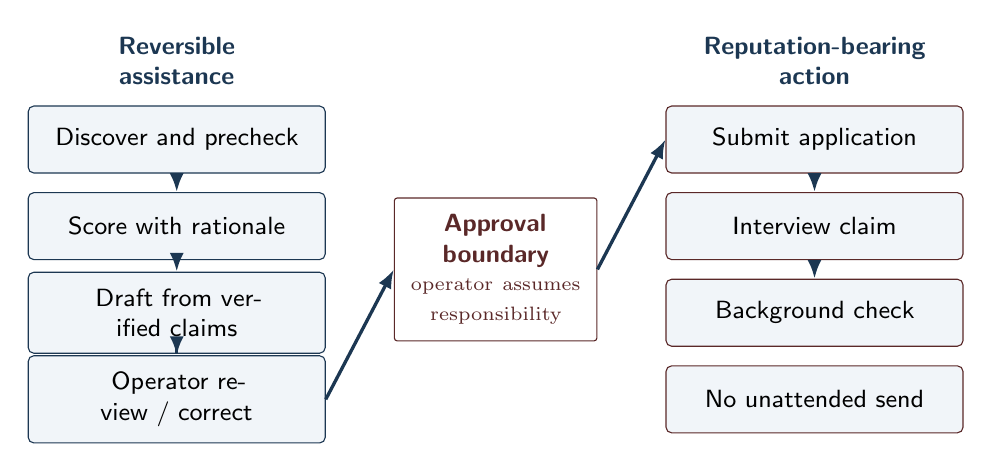
\begin{tikzpicture}[
  font=\small\sffamily,
  cell/.style={draw=zgink, fill=zgfill, rounded corners=2pt, align=center,
    inner sep=6pt, text width=3.35cm, minimum height=0.85cm},
  hdr/.style={font=\bfseries\sffamily\small, zgink, align=center, text width=3.4cm},
  arr/.style={-{Latex[length=2.4mm]}, zgink, very thick}
]
\node[hdr] (h1) at (0,2.55) {Reversible\\assistance};
\node[cell] (a1) at (0,1.55) {Discover and precheck};
\node[cell] (a2) at (0,0.45) {Score with rationale};
\node[cell] (a3) at (0,-0.65) {Draft from verified claims};
\node[cell] (a4) at (0,-1.75) {Operator review / correct};

\node[draw=zggate, fill=white, text=zggate, rounded corners=1pt, align=center,
  text width=2.15cm, inner sep=6pt, font=\bfseries\sffamily\small]
  (gate) at (4.05,-0.1) {Approval\\boundary\\[2pt]
  {\normalfont\scriptsize operator assumes\\responsibility}};

\node[hdr] (h2) at (8.1,2.55) {Reputation-bearing\\action};
\node[cell, draw=zggate] (b1) at (8.1,1.55) {Submit application};
\node[cell, draw=zggate] (b2) at (8.1,0.45) {Interview claim};
\node[cell, draw=zggate] (b3) at (8.1,-0.65) {Background check};
\node[cell, draw=zggate] (b4) at (8.1,-1.75) {No unattended send};

\draw[arr] (a1) -- (a2);
\draw[arr] (a2) -- (a3);
\draw[arr] (a3) -- (a4);
\draw[arr] (a4.east) -- (gate.west);
\draw[arr] (gate.east) -- (b1.west);
\draw[arr] (b1) -- (b2);
\draw[arr] (b2) -- (b3);
\end{tikzpicture}%
}
\caption{Risk heuristic. Model output may assist on the left, where errors are
cheap to catch. Crossing the approval boundary makes remaining errors
reputation-bearing. Supervision time belongs in the evaluation
\citep{liu2025agenticroi}; it is not a free safety layer.}
\label{fig:boundary}
\end{figure}

\section{A checklist for evaluating AI career-tool claims}
\label{sec:checklist}

(1) Outcome data, or testimonial --- and is the denominator (total
applications) reported? (2) Net of all costs, including subscription, review
time, and reputation risk? (3) What is $n$, and who selected the sample?
(4) Stratified by seniority, field, and market, or aggregate? (5) Measured,
or self-reported? (6) Who audits the number? (7) Is there a control arm ---
the same candidate, untailored or unassisted? (8) Would the vendor publish a
negative result? (This paper prospectively specifies its measurements and
commits to reporting failures so that item~8 is answered by construction.)

\section{Conclusion (provisional at v0.4)}

ZenGrowth is a working verification-first career tool, not only a proposed
architecture. It connects discovery, prioritization, evidence-grounded
materials, interview preparation, offers, and later lifecycle stages while
retaining reviewed evidence, deterministic checks for selected high-risk
tokens, telemetry, and operator approval before dispatch. The repository and
tests establish those useful capabilities. They do not yet quantify how smooth
or fast the workflow is, the rate at which unsupported semantic claims survive,
whether repeated scores are stable, or whether tailored materials improve
callbacks. Those are prospective tests, not conclusions. Layered rewrite
defenses with measured synthetic rates already exist
\citep{indukuri2026grounded}; what remains to be shown here is the operational
and outcome value of a live, denominator-complete field deployment.

The novelty claim is correspondingly narrow. Prior systems already generate
tailored resumes, retrieve from a career vault with provenance, and stack
deterministic rewrite defenses. ZenGrowth may contribute a longitudinal field
account connecting write-time controls, telemetry, correction burden, and
downstream outcomes. It will publish complete denominators. Whether that
contribution survives measurement is deliberately left open. At v0.4, the
strongest result is a functioning, integrated workflow with tested controls,
an explicit capability and outcome evidence ladder, and a falsifiable protocol
for measuring its correctness and effectiveness.

\paragraph{Planned revisions.} v1: execute and freeze the
Table~\ref{tab:pending} measurements, publish the claim-level adjudication
rubric, and report all aggregate results including failures. v2: add
tracked-campaign outcome data, an executable replay fixture, and the final
venue decision.

\subsubsection*{Reproducibility}
ZenGrowth's measurement protocol is documented in the repository
\citep{zengrowth2026protocol}. The deterministic eval gates that witness
architectural controls run in public CI. Dated aggregate baselines and their
derivation queries will be published with v1; underlying personal career data
will not be published (see Limitations).

\subsubsection*{Acknowledgments}
LLM-based coding and research tools assisted drafting, literature discovery,
and implementation inside the ZenGrowth repository. The author reviewed the
manuscript and accepts responsibility for its claims; empirical claims marked
unmeasured remain unresolved by design. The author is the system's sole
operator and beneficiary, which is both the evidence base and a declared
conflict. This work received no external funding.

\bibliographystyle{plainnat}
\small
\setlength{\bibsep}{2pt}
\bibliography{references}

\end{document}
